% ============================================================================
%  COMPILE WITH XeLaTeX  (twice, so the point total resolves)
%  Overleaf: Menu -> Compiler -> XeLaTeX
%  Requires: bnhandout.sty and fonts/Kalpurush.ttf in the project
% ============================================================================
\documentclass[11pt]{article}
\usepackage{bnhandout}          % add [nosol] for a student edition

\hauthor[https://sites.google.com/view/jugantordey/home]{Jugantor Dey}
\hseries{\textit{Mathematics for the Physics Olympiad}}

\begin{document}

\handouttitle{Chapter 19 : Ordinary Differential Equations}

\noindent
এই অধ্যায়ের ভিত্তি ১৭ নম্বর অধ্যায় (integral, প্রতিস্থাপন, অংশে অংশে
যোগজীকরণ) এবং ১৮ নম্বর অধ্যায় (Euler-এর সূত্র ও phasor)। ১৫ নম্বর
অধ্যায়ের derivative-এর নিয়ম আর ১৬ নম্বর অধ্যায়ের differential-এর
ভাষাও সারাক্ষণ লাগবে।

এখান থেকে সিরিজের Advanced অংশ শুরু। নাম দেখে ভয় পেয়ো না; নতুন কোনো
যন্ত্রপাতি লাগবে না, কেবল হাতে থাকা যন্ত্রগুলো একসঙ্গে ব্যবহার করতে হবে।

সিরিজজুড়ে বেশ কয়েকবার একটি প্রতিশ্রুতি দেওয়া হয়েছে। ১০ নম্বর অধ্যায়ে
সূচকীয় ক্ষয়ের প্রসঙ্গে বলা হয়েছিল যে ``পরিবর্তনের হার নিজের পরিমাণের
সমানুপাতিক'' কথাটির গাণিতিক রূপ $\dfrac{dN}{dt} = kN$, আর সেখান থেকে
$N = N_{0}e^{kt}$ বের করার কাজটি ১৯ নম্বর অধ্যায়ের। ১২ নম্বর অধ্যায়ে
গ্রহের কক্ষপথের প্রসঙ্গে একই কথা। ১৮ নম্বর অধ্যায়ে বলা হয়েছিল যে
$e^{i\omega t}$ ব্যবহার করে দোলনের সমীকরণকে বীজগণিতে নামিয়ে আনা যায়, আর
সেটিও এখানে। এই অধ্যায়ে সব কটি ধার শোধ হবে।

মূল ধারণাটি এক বাক্যে বলা যায়। বীজগণিতের সমীকরণে অজানা একটি \emph{সংখ্যা};
অন্তরক সমীকরণে অজানা একটি \emph{ফাংশন}, আর সমীকরণটি ওই ফাংশনের পরিবর্তনের হার
সম্পর্কে একটি বিবৃতি। পদার্থবিজ্ঞান প্রায় পুরোটাই এই ভাষায় লেখা, কারণ
প্রকৃতির নিয়মগুলো সরাসরি অবস্থান বলে দেয় না; তারা বলে দেয় কোন হারে কী বদলাবে।
Newton-এর দ্বিতীয় সূত্র $F = m\ddot{x}$ ঠিক এই ধরনের একটি বিবৃতি।

এই অধ্যায়ে মোট \totalpoints\ পয়েন্ট আছে।

\section{ODE কী}

\begin{idea}[অন্তরক সমীকরণ ও তার সমাধান]
একটি অজানা ফাংশন এবং তার derivative-গুলো নিয়ে লেখা সমীকরণকে বলে differential
equation। স্বাধীন চলক একটিমাত্র হলে তাকে বলে ordinary differential equation,
সংক্ষেপে ODE।

কোনো ফাংশনকে সমাধান বলা হয় যদি সেটি সমীকরণে বসালে দুই পাশ সমান হয়। সাধারণত
সমাধান একটি নয়, একটি \emph{পরিবার}; পরিবার থেকে একটিকে বেছে নেয় initial
condition।
\end{idea}

উদাহরণ দিয়ে দেখা যাক। $\dfrac{dy}{dx} = -y$ সমীকরণটি বলছে: এমন একটি ফাংশন খোঁজো
যার derivative তার নিজেরই ঋণাত্মক। ১৫ নম্বর অধ্যায় থেকে জানি
$\dfrac{d}{dx}e^{-x} = -e^{-x}$, তাই $y = e^{-x}$ কাজ করে। কিন্তু
$y = Ce^{-x}$-ও কাজ করে, যেকোনো ধ্রুবক $C$-এর জন্য।

\begin{center}
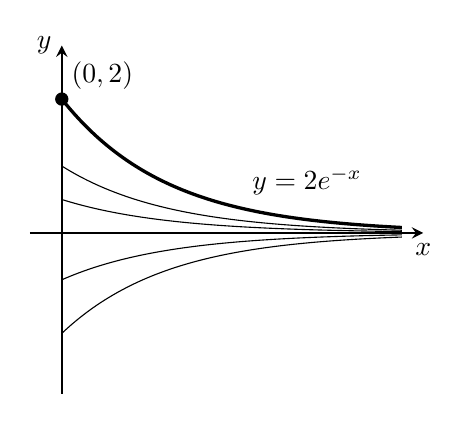
\begin{tikzpicture}[x=1.35cm,y=0.85cm,>=stealth]
  \draw[thick,->] (-0.3,0) -- (3.4,0) node[below] {$x$};
  \draw[thick,->] (0,-2.4) -- (0,2.8) node[left] {$y$};
  \foreach \C in {1,0.5,-0.7,-1.5}{
    \draw[thin,domain=0:3.2,samples=80,variable=\x] plot ({\x},{\C*exp(-\x)});
  }
  \draw[very thick,domain=0:3.2,samples=80,variable=\x] plot ({\x},{2*exp(-\x)});
  \draw[fill] (0,2) circle (2.2pt) node[above right] {$(0,2)$};
  \node[right] at (1.7,0.78) {$y=2e^{-x}$};
\end{tikzpicture}
\end{center}

ছবিতে ওই পরিবারের কয়েকজন সদস্য আঁকা। কেউ একজন যদি বলে দেয় $y(0) = 2$, তবে
$C = 2$ ঠিক হয়ে যায় এবং একটিমাত্র বক্ররেখা বাকি থাকে (মোটা রেখাটি)।

\begin{idea}[সাধারণ ও বিশেষ সমাধান]
$n$ ক্রমের ODE-এর সাধারণ সমাধানে সাধারণত $n$টি স্বাধীন ধ্রুবক থাকে, আর একটি
নির্দিষ্ট সমাধান বেছে নিতে $n$টি শর্ত লাগে। শর্তগুলো একই বিন্দুতে দেওয়া হলে
তাদের বলে initial condition; আলাদা দুই প্রান্তে দেওয়া হলে boundary condition।
\end{idea}

কেন $n$টি ধ্রুবক লাগে, তা বোঝা সহজ: প্রতিবার integrate করলে একটি করে
$+C$ আসে (১৭ নম্বর অধ্যায়), আর $n$ ক্রমের সমীকরণ কার্যত $n$ বার integrate
করার সমান। এই বাক্যটির একটি নির্ভুল রূপ আছে যা
এই সিরিজে প্রমাণ করা হচ্ছে না; ফিজিক্স অলিম্পিয়াডেও লাগবে না সাধারণত। 

\begin{example}
দেখাও যে $y = A\sin 2x + B\cos 2x$ সব $A, B$-এর জন্য $y'' + 4y = 0$
সমীকরণটি সিদ্ধ হয় । তারপর $y(0) = 1$, $y'(0) = 6$ শর্তে $A$ ও $B$ নির্ণয় করো।
\end{example}

\begin{solbox}
Derivative নিই:
\[
  y' = 2A\cos 2x - 2B\sin 2x, \qquad
  y'' = -4A\sin 2x - 4B\cos 2x = -4y .
\]
সুতরাং $y'' + 4y = 0$, যেকোনো $A, B$-এর জন্য।

শর্ত বসাই: $y(0) = B = 1$, আর $y'(0) = 2A = 6$ দেয় $A = 3$। সুতরাং
\[
  y = 3\sin 2x + \cos 2x .
\]
দুই ক্রমের সমীকরণ, দুটি ধ্রুবক, দুটি শর্ত। হিসাব মিলছে।
\end{solbox}

\prob{3} $y = \dfrac{1}{C-x}$ ফাংশনটি $y' = y^{2}$ সমীকরণের সমাধান, দেখাও।
$y(0) = 1$ শর্তে সমাধানটি লেখো এবং তার একটি বিস্ময়কর বৈশিষ্ট্য বলো।

\begin{sol}
$y = (C-x)^{-1}$ ধরে chain rule প্রয়োগ করি:
\[
  y' = -(C-x)^{-2} \cdot (-1) = \frac{1}{(C-x)^{2}} = y^{2} .
\]
সুতরাং সমাধান।

$y(0) = \dfrac{1}{C} = 1$ দেয় $C = 1$, অর্থাৎ
\[
  y = \frac{1}{1-x} .
\]
বৈশিষ্ট্য: $x \to 1^{-}$-এ $y \to \infty$। অর্থাৎ সমাধানটি সসীম সময়েই ভেঙে
পড়ে, যদিও সমীকরণটি দেখতে নিরীহ এবং সর্বত্র সংজ্ঞায়িত। একে বলে finite-time
blow-up।

শিক্ষণীয়: ODE-এর সমাধান সবসময় সব $x$-এর জন্য থাকে না। রৈখিক সমীকরণে এই
সমস্যা হয় না, কিন্তু $y^{2}$ পদটি অরৈখিক (১৪ নম্বর অধ্যায়), আর
অরৈখিকতাই এই আচরণের উৎস।
\end{sol}

\prob{3} $y'' - y = 0$ সমীকরণটির জন্য
\begin{enumerate}
  \item দেখাও যে $y = Ae^{x} + Be^{-x}$ একটি সমাধান;
  \item দেখাও যে $y = P\cosh x + Q\sinh x$-ও একটি সমাধান (১০ নম্বর
        অধ্যায়);
  \item ব্যাখ্যা করো কেন এই দুটি আসলে একই সমাধান-।
\end{enumerate}

\begin{sol}
\begin{enumerate}
  \item $y'' = Ae^{x} + Be^{-x} = y$, তাই $y'' - y = 0$।
  \item ১৭ নম্বর অধ্যায়ে দেখা গেছে $\cosh' = \sinh$ ও $\sinh' = \cosh$,
        তাই দুবার derivative নিলে দুটোই নিজেদের ফিরে পায়:
        $y'' = P\cosh x + Q\sinh x = y$।
  \item সংজ্ঞা অনুযায়ী $\cosh x = \dfrac{e^{x}+e^{-x}}{2}$ ও
        $\sinh x = \dfrac{e^{x}-e^{-x}}{2}$, তাই
        \[
          P\cosh x + Q\sinh x
          = \frac{P+Q}{2}e^{x} + \frac{P-Q}{2}e^{-x} .
        \]
        অর্থাৎ $A = \dfrac{P+Q}{2}$, $B = \dfrac{P-Q}{2}$ বসালেই প্রথম রূপটি
        পাওয়া যায়, আর উল্টোটাও করা যায় ($P = A+B$, $Q = A-B$)। দুটি ভিন্ন
        নাম, একই দুই-পরামিতির পরিবার।
\end{enumerate}
কোন রূপটি সুবিধাজনক তা নির্ভর করে শর্তের উপর: $x=0$-এ শর্ত দেওয়া থাকলে
$\cosh$-$\sinh$ রূপ সহজ, কারণ $\cosh 0 = 1$ ও $\sinh 0 = 0$।
\end{sol}

\section{ক্রম ও ঘাত}

শ্রেণীবিভাগ শুনতে নীরস, কিন্তু কাজে লাগে: কোন কৌশল খাটবে তা প্রায় পুরোটাই
নির্ভর করে সমীকরণটি কোন শ্রেণির।

\begin{idea}[ক্রম, ঘাত ও রৈখিকতা]
\textbf{ক্রম (order)}: সমীকরণে উপস্থিত সর্বোচ্চ derivative-এর ক্রম।

\textbf{ঘাত (degree)}: মূল ও ভগ্নাংশ সরিয়ে সমীকরণটিকে derivative-গুলোর
বহুপদী আকারে আনার পর সর্বোচ্চ derivative-এর ঘাত। বহুপদী আকারে আনা না গেলে
ঘাত সংজ্ঞায়িত নয়।

\textbf{রৈখিক (linear)}: $y$ ও তার derivative-গুলো কেবল প্রথম ঘাতে আছে এবং
তাদের মধ্যে কোনো গুণ নেই, অর্থাৎ সমীকরণটি
\[
  a_{n}(x)y^{(n)} + \cdots + a_{1}(x)y' + a_{0}(x)y = f(x)
\]
আকারে লেখা যায়। সহগগুলো $x$-এর যত জটিল ফাংশনই হোক, তাতে রৈখিকতা নষ্ট হয় না।
\end{idea}

তিনটির মধ্যে রৈখিকতাই সবচেয়ে গুরুত্বপূর্ণ, আর কেন তা পরের অনুচ্ছেদে দেখা
যাবে। ঘাত বরং কম গুরুত্বপূর্ণ; স্কুলের শ্রেণীবিভাগে এর জায়গা আছে, কিন্তু
সমাধানের কৌশল বাছতে তা খুব কমই লাগে।

\begin{example}
$\sqrt{1 + (y')^{2}} = y''$ সমীকরণটির ক্রম ও ঘাত নির্ণয় করো।
\end{example}

\begin{solbox}
সর্বোচ্চ derivative $y''$, তাই ক্রম $2$।

ঘাত বের করতে আগে মূল সরাতে হবে। দুই পাশ বর্গ করি:
\[
  1 + (y')^{2} = (y'')^{2} .
\]
এখন সমীকরণটি derivative-গুলোর বহুপদী, আর $y''$-এর সর্বোচ্চ ঘাত $2$। সুতরাং
ঘাত $2$।

রৈখিক কি? না। $(y'')^{2}$ ও $(y')^{2}$ দুটিই দ্বিতীয় ঘাতে আছে।

(বাস্তবে এই সমীকরণটি একটি জ্যামিতিক প্রশ্ন থেকে আসে; ১৭ নম্বর অধ্যায়ের
চাপের উপাদানের সঙ্গে মিলিয়ে দেখো, বাম পাশটি ঠিক $ds/dx$।)
\end{solbox}

\prob{3} নিচের প্রতিটির ক্রম, ঘাত ও রৈখিকতা নির্ণয় করো।
\begin{enumerate}
  \item $y'' + 3y' + 2y = \sin x$
  \item $(y')^{2} + y = 0$
  \item $y'' + y\,y' = 0$
  \item $x^{2}y'' + e^{x}y = \ln x$
\end{enumerate}

\begin{sol}
\begin{enumerate}
  \item ক্রম $2$, ঘাত $1$, রৈখিক। ডান পাশে $\sin x$ থাকায় রৈখিকতা নষ্ট হয়
        না, কারণ সেটি $y$-এর উপর নির্ভর করে না।
  \item ক্রম $1$, ঘাত $2$, অরৈখিক।
  \item ক্রম $2$, ঘাত $1$, কিন্তু অরৈখিক: $y\,y'$ পদে অজানা ফাংশন ও তার
        derivative গুণ হয়ে আছে।
  \item ক্রম $2$, ঘাত $1$, রৈখিক। সহগ $x^{2}$ ও $e^{x}$ যতই জটিল হোক, তারা
        কেবল $x$-এর ফাংশন, তাই রৈখিকতা অক্ষুণ্ন।
\end{enumerate}
তৃতীয় ও চতুর্থটি পাশাপাশি রাখলে পার্থক্যটা পরিষ্কার হয়: সহগে জটিলতা চলে,
$y$-এর সঙ্গে $y$-এর গুণ চলে না।
\end{sol}

\section{সমসত্ত্বতা}

\begin{idea}[সমসত্ত্ব ও অসমসত্ত্ব]
ধারণা ৩-এর রৈখিক সমীকরণে $f(x) = 0$ হলে তাকে বলে homogeneous, নইলে
inhomogeneous।
\end{idea}

\begin{remark}
সাবধান, ``homogeneous'' শব্দটির আরেকটি অর্থও প্রচলিত: কিছু বইয়ে
$\dfrac{dy}{dx} = F\left( \dfrac{y}{x} \right)$ আকারের প্রথম ক্রমের সমীকরণকেও
homogeneous বলা হয়। দুটি অর্থ সম্পূর্ণ আলাদা। এই অধ্যায়ে সবসময় উপরের
অর্থটাই ব্যবহার করা হবে, অর্থাৎ ডান পাশ শূন্য।
\end{remark}

এবার রৈখিকতার আসল পুরস্কার।

\begin{idea}[উপরিপাতন (superposition)]
$y_{1}$ ও $y_{2}$ যদি একটি রৈখিক \emph{সমসত্ত্ব} সমীকরণের সমাধান হয়, তবে
যেকোনো ধ্রুবক $c_{1}, c_{2}$-এর জন্য $c_{1}y_{1} + c_{2}y_{2}$-ও সমাধান।
\end{idea}

প্রমাণ দুই লাইনের। সমীকরণটি সংক্ষেপে $L[y] = 0$ লিখি, যেখানে
$L[y] = a_{n}y^{(n)} + \cdots + a_{0}y$। Derivative নেওয়া রৈখিক (১৫ নম্বর
অধ্যায়ের প্রথম নিয়ম), তাই
\[
  L\left[ c_{1}y_{1} + c_{2}y_{2} \right]
  = c_{1}L[y_{1}] + c_{2}L[y_{2}] = c_{1} \cdot 0 + c_{2} \cdot 0 = 0 .
\]

১৪ নম্বর অধ্যায়ের শেষ অনুচ্ছেদে বলা হয়েছিল যে রৈখিক জিনিস নিয়ে কাজ করা
সহজ, কারণ জটিল ইনপুটকে সরল ইনপুটের যোগফলে ভেঙে ফেলা যায়। উপরের ফলটিই সেই
কথার সবচেয়ে গুরুত্বপূর্ণ প্রয়োগ, আর তরঙ্গের উপরিপাতন থেকে শুরু করে বর্তনীর
বিশ্লেষণ পর্যন্ত সবই এর উপর দাঁড়ানো।

\begin{idea}[অসমসত্ত্ব সমীকরণের গঠন]
$L[y] = f$ সমীকরণের সাধারণ সমাধান সবসময় দুটি অংশের যোগফল:
\[
  y = y_{p} + y_{c} .
\]
\textbf{বিশেষ সমাধান} $y_{p}$ (particular solution): মূল সমীকরণ $L[y] = f$-এর
যেকোনো \emph{একটি} সমাধান, যাতে কোনো অনির্দিষ্ট ধ্রুবক নেই। কোনটি নিলে, তাতে
কিছু যায় আসে না।

\textbf{Complementary function} $y_{c}$: ডান পাশ শূন্য করে পাওয়া সমসত্ত্ব
সমীকরণ $L[y] = 0$-এর সাধারণ সমাধান। $n$ ক্রমের সমীকরণের $n$টি অনির্দিষ্ট ধ্রুবক
সবই থাকে এই অংশে।
\end{idea}

এর ফলে একটি কঠিন কাজ দুটি সহজ কাজে ভাগ হয়ে যায়। এক, যেকোনো উপায়ে (দরকার হলে
অনুমান করে) $L[y] = f$-এর মাত্র একটি সমাধান খুঁজে বের করা। দুই, সমসত্ত্ব
সমীকরণটি পুরোপুরি সমাধান করা। তারপর দুটো যোগ করলেই কাজ শেষ।

কথাটি কেন সত্য, তা দেখাতে দুটি জিনিস প্রমাণ করতে হবে। দুটিতেই একমাত্র হাতিয়ার
$L$-এর রৈখিকতা, যা উপরিপাতনের প্রমাণে ব্যবহার করেছি।

\textbf{প্রথমত, এই আকারের প্রতিটি ফাংশনই সমাধান।} যেহেতু $L[y_{p}] = f$ এবং
$L[y_{c}] = 0$,
\[
  L[y_{p} + y_{c}] = L[y_{p}] + L[y_{c}] = f + 0 = f .
\]

\textbf{দ্বিতীয়ত, এর বাইরে কোনো সমাধান নেই।} ধরো $y$ যেকোনো একটি সমাধান, অর্থাৎ
$L[y] = f$। তাহলে
\[
  L[y - y_{p}] = L[y] - L[y_{p}] = f - f = 0 .
\]
অর্থাৎ $y - y_{p}$ সমসত্ত্ব সমীকরণের একটি সমাধান, তাই সেটি $y_{c}$ পরিবারেরই
কোনো একজন সদস্য। সুতরাং যেকোনো সমাধান $y$ আসলে $y_{c}$-এর একজন
সদস্য আর $y_{p}$-এর যোগফল, অন্য কিছু নয়।

দ্বিতীয় যুক্তিটি থেকে আরেকটি কথা বেরিয়ে আসে। দুটি ভিন্ন বিশেষ সমাধানের
পার্থক্যও সমসত্ত্ব সমীকরণের সমাধান, তাই সেই পার্থক্যটুকু $y_{c}$-এর ধ্রুবকের
মধ্যে মিশে যায়। যেমন নিচের উদাহরণের $y'' + y = x$ সমীকরণে $y_{p} = x$-এর
বদলে $y_{p} = x + \sin x$ নিলেও চলে (বসিয়ে যাচাই করো), আর তখন উত্তর দাঁড়ায়
$y = x + A\cos x + (B+1)\sin x$। এটি একই পরিবার, কেবল $B$-এর জায়গায় $B+1$
লেখা। তাই $y_{p}$ হিসেবে সবসময় হাতের কাছের সবচেয়ে সরলটিই নাও।


\begin{example}
$y'' + y = x$ সমীকরণের একটি বিশেষ সমাধান $y_{p} = x$, যাচাই করো এবং সাধারণ
সমাধান লেখো।
\end{example}

\begin{solbox}
যাচাই: $y_{p} = x$ হলে $y_{p}'' = 0$, তাই $y_{p}'' + y_{p} = 0 + x = x$।
ঠিক আছে।

সমসত্ত্ব সমীকরণ $y'' + y = 0$-এর সাধারণ সমাধান $A\cos x + B\sin x$ (প্রথম
অনুচ্ছেদের উদাহরণের মতোই, কেবল $2$-এর জায়গায় $1$)। সুতরাং
\[
  y = x + A\cos x + B\sin x .
\]
\end{solbox}

\prob{3} উপরিপাতন উপপাদ্যটি প্রমাণ করো, এবং একটি উদাহরণ দিয়ে দেখাও যে
অরৈখিক সমীকরণে এটি ভেঙে পড়ে।

\begin{sol}
প্রমাণ উপরে দেওয়া হয়েছে: $L$ রৈখিক হওয়ায়
$L[c_{1}y_{1}+c_{2}y_{2}] = c_{1}L[y_{1}] + c_{2}L[y_{2}] = 0$।

ভেঙে পড়ার উদাহরণ: $y' = y^{2}$ নাও, যা অরৈখিক। প্রথম সমস্যা থেকে জানি
$y_{1} = \dfrac{1}{1-x}$ একটি সমাধান। এখন $2y_{1}$ কি সমাধান? বাম পাশ
$(2y_{1})' = 2y_{1}' = 2y_{1}^{2}$, আর ডান পাশ $(2y_{1})^{2} = 4y_{1}^{2}$।
দুটি সমান নয় (যেখানে $y_{1} \neq 0$)। সুতরাং ধ্রুবক দিয়ে গুণ করলেও সমাধান
থাকে না, যোগ করা তো দূরের কথা।

এই কারণেই অরৈখিক সমীকরণ এত কঠিন: সমাধান ভেঙে ভেঙে গড়ে তোলার উপায় থাকে না।
\end{sol}

\prob{4} $y'' + y = x$ সমীকরণের সাধারণ সমাধান থেকে $y(0) = 0$, $y'(0) = 0$
শর্তে বিশেষ সমাধান নির্ণয় করো, এবং ছোট $x$-এর জন্য উত্তরটি কেমন আচরণ করে তা
বলো।

\begin{sol}
সাধারণ সমাধান $y = x + A\cos x + B\sin x$।

$y(0) = 0 + A = 0$ দেয় $A = 0$।

$y' = 1 - A\sin x + B\cos x$, তাই $y'(0) = 1 + B = 0$ দেয় $B = -1$। সুতরাং
\[
  y = x - \sin x .
\]

ছোট $x$-এর আচরণ: ১৫ নম্বর অধ্যায়ের Taylor সিরিজ থেকে
$\sin x = x - \dfrac{x^{3}}{6} + \cdots$, তাই
\[
  y = x - \sin x = \frac{x^{3}}{6} - \cdots
\]
অর্থাৎ শুরুতে $y$ প্রায় $x^{3}/6$ হয়ে বাড়ে, খুব ধীরে। শর্ত দুটি মান ও ঢাল
দুটোকেই শূন্য করে দিয়েছে, তাই প্রথম অশূন্য পদটি তৃতীয় ঘাতে গিয়ে দেখা দিল।
\end{sol}

\section{নোটেশন}

একই জিনিস অনেক রকমে লেখা হয়, আর বই বদলালে নোটেশনও বদলায়। চেনা থাকা দরকার।

\begin{idea}[চারটি লেখার ভঙ্গি]
\[
  y', \; y'', \; y^{(n)}, \qquad
  \frac{dy}{dx}, \; \frac{d^{2}y}{dx^{2}}, \qquad
  \dot{x}, \; \ddot{x}, \qquad
  Dy, \; D^{2}y .
\]
এরা যথাক্রমে Lagrange, Leibniz, Newton ও operator নোটেশন। Newton-এর বিন্দু
সবসময় সময়ের সাপেক্ষে derivative বোঝায়, আর operator ভঙ্গিতে
$D = \dfrac{d}{dx}$ ধরা হয়।
\end{idea}

Operator রূপটি বিশেষভাবে কাজের। $y'' + 5y' + 6y = 0$ লেখা যায়
\[
  \left( D^{2} + 5D + 6 \right)y = 0 ,
\]
আর ধ্রুবক সহগ থাকলে বন্ধনীর ভেতরের রাশিটিকে সাধারণ বহুপদীর মতো উৎপাদকে
বিশ্লেষণ করা যায়:
\[
  \left( D+2 \right)\left( D+3 \right)y = 0 .
\]
এটি বৈধ কারণ ধ্রুবক সহগের ক্ষেত্রে $D$ ও ধ্রুবক পরস্পর বিনিময়যোগ্য, তাই
বন্ধনী খুললে মূল রাশিটিই ফিরে আসে (হাতে খুলে যাচাই করে দেখো)। সহগ $x$-এর
ফাংশন হলে এই সরলতা থাকে না; তখন $D$ ও সহগ বিনিময়যোগ্য নয়।

\begin{remark}
একটি সীমারেখা টেনে রাখি। ODE-তে স্বাধীন চলক একটিমাত্র। একাধিক স্বাধীন চলক
থাকলে derivative-গুলো আংশিক হয়ে যায় (১৫ নম্বর অধ্যায়) এবং সমীকরণটিকে বলা
হয় partial differential equation। তরঙ্গ সমীকরণ, তাপ সমীকরণ ও Maxwell-এর
সমীকরণ সবই PDE। এই সিরিজে PDE সমাধান করা হবে না; ২১ নম্বর অধ্যায়ে কেবল
তাদের লেখার ভাষাটুকু তৈরি হবে।
\end{remark}

\begin{example}
$\left( D^{2} - 4 \right)y = 0$ সমীকরণটি উৎপাদকে বিশ্লেষণ করে সমাধান করো।
\end{example}

\begin{solbox}
\[
  \left( D-2 \right)\left( D+2 \right)y = 0 .
\]
$(D+2)y = 0$ হলে $y' = -2y$, যার সমাধান $y = Be^{-2x}$। আবার
$(D-2)y = 0$ হলে $y = Ae^{2x}$। দুটিই সমাধান, আর সমীকরণটি রৈখিক ও সমসত্ত্ব,
তাই উপরিপাতন অনুযায়ী
\[
  y = Ae^{2x} + Be^{-2x} .
\]
দুই ক্রমের সমীকরণে দুটি ধ্রুবক এসেছে, যা প্রত্যাশিত। এটিই সব সমাধান কি না,
সেই দাবিটি অস্তিত্ব-ও-অদ্বিতীয়তা উপপাদ্যের উপর দাঁড়ানো, যা আমরা ধরে নিচ্ছি।
\end{solbox}

\prob{3} $y'' + 5y' + 6y = 0$ সমীকরণটিকে operator আকারে লিখে উৎপাদকে বিশ্লেষণ
করো, এবং সাধারণ সমাধান নির্ণয় করো। এরপর $y(0) = 1$, $y'(0) = 0$ শর্তে বিশেষ
সমাধান বের করো।

\begin{sol}
\[
  \left( D^{2}+5D+6 \right)y = \left( D+2 \right)\left( D+3 \right)y = 0 ,
\]
তাই সাধারণ সমাধান $y = Ae^{-2x} + Be^{-3x}$।

শর্ত বসাই: $y(0) = A + B = 1$ এবং $y' = -2Ae^{-2x} - 3Be^{-3x}$ থেকে
$y'(0) = -2A - 3B = 0$।

দ্বিতীয়টি থেকে $A = -\tfrac{3}{2}B$; প্রথমটিতে বসিয়ে
$-\tfrac{3}{2}B + B = 1$, অর্থাৎ $-\tfrac{1}{2}B = 1$, তাই $B = -2$ ও
$A = 3$। সুতরাং
\[
  y = 3e^{-2x} - 2e^{-3x} .
\]
যাচাই: $y(0) = 3-2 = 1$ এবং $y'(0) = -6+6 = 0$। ঠিক আছে।
\end{sol}

\section{সমাধানের কৌশল}

তিনটি কৌশলে অলিম্পিয়াডে যা যা লাগে তার প্রায় সবই কুলিয়ে যায়।

\begin{idea}[কৌশল ১: চলক পৃথকীকরণ (seperating variables)]
$\dfrac{dy}{dx} = g(x)h(y)$ আকারের সমীকরণে দুই চলককে দুই পাশে সরিয়ে নাও:
\[
  \frac{dy}{h(y)} = g(x)\,dx ,
\]
তারপর দুই পাশে integrate করো।
\end{idea}

এই ধাপটা দেখতে অবৈধ লাগতে পারে, তাই কেন বৈধ সেটা বলে রাখি। ১৬ নম্বর
অধ্যায় অনুযায়ী $dy$ ও $dx$ সত্যিকারের রাশি, আর $dy = y'\,dx$। মূল
সমীকরণকে $\dfrac{1}{h(y)}\dfrac{dy}{dx} = g(x)$ লিখে দুই পাশকে $x$-এর সাপেক্ষে
integrate করলে বাম পাশে ১৭ নম্বর অধ্যায়ের প্রতিস্থাপনের নিয়ম প্রয়োগ করা
যায় এবং ঠিক $\int \dfrac{dy}{h(y)}$ পাওয়া যায়। সাবধানতা: $h(y) = 0$ হলে ভাগ
করা যায় না, আর ওই ধ্রুবক সমাধানগুলো আলাদা করে দেখতে হয়।

\begin{example}
১০ নম্বর অধ্যায়ের ধার শোধ করো: $\dfrac{dN}{dt} = kN$ সমীকরণটি
$N(0) = N_{0}$ শর্তে সমাধান করো।
\end{example}

\begin{solbox}
প্রথমে $N \equiv 0$ ধ্রুবক সমাধানটি আলাদা করে রাখি; সেটিও সমীকরণ মেটায়।
এখন $N \neq 0$ ধরে চলক পৃথক করি:
\[
  \frac{dN}{N} = k\,dt .
\]
দুই পাশে integrate করি (১৭ নম্বর অধ্যায়ের তালিকা):
\[
  \ln|N| = kt + C_{1} .
\]
দুই পাশে $\exp$ নিয়ে $|N| = e^{C_{1}}e^{kt}$, অর্থাৎ $N = Ce^{kt}$ যেখানে
$C = \pm e^{C_{1}}$ যেকোনো অশূন্য ধ্রুবক। ($C = 0$ নিলে বাদ রাখা ধ্রুবক
সমাধানটিও ঢুকে পড়ে, তাই সব মিলিয়ে $C$ যেকোনো বাস্তব সংখ্যা।)

শর্ত: $N(0) = C = N_{0}$। সুতরাং
\[
  N(t) = N_{0}e^{kt} .
\]
১০ নম্বর অধ্যায়ে এই রূপটিকে সংজ্ঞা ধরে নিয়ে কাজ চালানো হয়েছিল এবং বলা
হয়েছিল যে ``সমান ব্যবধিতে সমান গুণিতক'' আর ``হার পরিমাণের সমানুপাতিক'' দুটি
বর্ণনা একই; এখন সেটি প্রমাণিত।
\end{solbox}

\begin{idea}[কৌশল ২: সমাকলন গুণক (Integrating factor)    ]
প্রথম ক্রমের রৈখিক সমীকরণ
\[
  y' + P(x)y = Q(x)
\]
সমাধান করতে দুই পাশকে $\mu(x) = e^{\int P\,dx}$ দিয়ে গুণ করো। তখন বাম পাশ
হয়ে যায় $\left( \mu y \right)'$, এবং
\[
  \mu y = \int \mu Q\,dx + C .
\]
\end{idea}

কেন কাজ করে: product rule অনুযায়ী $(\mu y)' = \mu y' + \mu' y$, আর
$\mu = e^{\int P dx}$ নিলে chain rule দেয় $\mu' = P\mu$। সুতরাং
$(\mu y)' = \mu\left( y' + Py \right) = \mu Q$। গোটা কৌশলটি আসলে product
rule-কে উল্টো দিক থেকে পড়া।

\begin{idea}[কৌশল ৩: ধ্রুবক সহগের দ্বিতীয় ক্রম]
$ay'' + by' + cy = 0$ সমাধান করতে $y = e^{\lambda t}$ বসাও। তখন
\[
  \left( a\lambda^{2} + b\lambda + c \right)e^{\lambda t} = 0 ,
\]
আর $e^{\lambda t} \neq 0$ বলে
\[
  a\lambda^{2} + b\lambda + c = 0 .
\]
একে বলে characteristic equation। তিনটি ক্ষেত্র:
\begin{enumerate}
  \item দুটি আলাদা বাস্তব মূল $\lambda_{1}, \lambda_{2}$:
        $y = Ae^{\lambda_{1}t} + Be^{\lambda_{2}t}$।
  \item জটিল মূল $\lambda = \alpha \pm i\beta$:
        $y = e^{\alpha t}\left( A\cos\beta t + B\sin\beta t \right)$।
  \item পুনরাবৃত্ত মূল $\lambda$:
        $y = \left( A + Bt \right)e^{\lambda t}$।
\end{enumerate}
\end{idea}

দ্বিতীয় ক্ষেত্রটিতে ১৮ নম্বর অধ্যায় কাজে লাগে। জটিল মূল থেকে পাওয়া
$e^{(\alpha+i\beta)t} = e^{\alpha t}e^{i\beta t}$, আর Euler-এর সূত্র বলছে
$e^{i\beta t} = \cos\beta t + i\sin\beta t$। দুটি জটিল সমাধানের যোগ ও বিয়োগ
নিয়ে (উপরিপাতন) বাস্তব সমাধান দুটি বেরিয়ে আসে। ১৮ নম্বর অধ্যায়ে বলা
হয়েছিল যে জটিল সংখ্যা দিয়ে দোলনের হিসাব সহজ হয়; এটিই তার প্রথম প্রমাণ।

তৃতীয় ক্ষেত্রে $te^{\lambda t}$ কোথা থেকে এল তা সরাসরি বসিয়ে যাচাই করা যায়
(শেষ অনুচ্ছেদের একটি সমস্যা), তবে তিনটি ক্ষেত্রেই ``এই দুই-পরামিতির পরিবারই
সব সমাধান'' দাবিটি অস্তিত্ব-ও-অদ্বিতীয়তা উপপাদ্যের উপর দাঁড়ানো, যা এখানে
ধরে নেওয়া হচ্ছে।

\begin{example}
$y' + \dfrac{2}{x}y = x$ সমীকরণটি সমাকলন গুণক দিয়ে সমাধান করো ($x > 0$)।
\end{example}

\begin{solbox}
এখানে $P = \dfrac{2}{x}$, তাই
\[
  \int P\,dx = 2\ln x = \ln x^{2}
  \;\Longrightarrow\; \mu = e^{\ln x^{2}} = x^{2} .
\]
দুই পাশকে $x^{2}$ দিয়ে গুণ করি:
\[
  x^{2}y' + 2xy = x^{3}
  \;\Longrightarrow\; \left( x^{2}y \right)' = x^{3} .
\]
Integrate করে
\[
  x^{2}y = \frac{x^{4}}{4} + C
  \;\Longrightarrow\; y = \frac{x^{2}}{4} + \frac{C}{x^{2}} .
\]
যাচাই: $y' = \dfrac{x}{2} - \dfrac{2C}{x^{3}}$, তাই
$y' + \dfrac{2}{x}y = \dfrac{x}{2} - \dfrac{2C}{x^{3}} + \dfrac{x}{2}
+ \dfrac{2C}{x^{3}} = x$। ঠিক আছে।
\end{solbox}

\prob{3} চলক পৃথকীকরণ ব্যবহার করে সমাধান করো: $\dfrac{dy}{dx} = xy$,
$y(0) = 2$।

\begin{sol}
$y \equiv 0$ একটি ধ্রুবক সমাধান, কিন্তু শর্তটি তা বাতিল করে। $y \neq 0$ ধরে
\[
  \frac{dy}{y} = x\,dx
  \;\Longrightarrow\; \ln|y| = \frac{x^{2}}{2} + C_{1}
  \;\Longrightarrow\; y = Ce^{x^{2}/2} .
\]
$y(0) = C = 2$, সুতরাং
\[
  y = 2e^{x^{2}/2} .
\]
যাচাই: $y' = 2e^{x^{2}/2}\cdot x = xy$। ঠিক আছে।
\end{sol}

\prob{3} একটি বস্তু বাতাসে পড়ছে এবং তার উপর বাধা বেগের সমানুপাতিক, তাই
\[
  \frac{dv}{dt} = g - kv, \qquad v(0) = 0 .
\]
সমাধান করো এবং প্রান্তিক বেগ (terminal velocity) নির্ণয় করো।

\begin{sol}
চলক পৃথক করি ($v \neq g/k$ ধরে):
\[
  \frac{dv}{g-kv} = dt .
\]
বাম পাশে $u = g-kv$ প্রতিস্থাপন করি, $du = -k\,dv$:
\[
  -\frac{1}{k}\ln|g-kv| = t + C_{1} .
\]
সাজিয়ে $g - kv = Ce^{-kt}$। শর্ত $v(0)=0$ দেয় $C = g$, তাই
\[
  v(t) = \frac{g}{k}\left( 1 - e^{-kt} \right) .
\]
প্রান্তিক বেগ: $t$ বড় হলে $e^{-kt} \to 0$, তাই $v \to \dfrac{g}{k}$।

দ্রুত যাচাই: প্রান্তিক অবস্থায় ত্বরণ শূন্য, অর্থাৎ $g = kv$, যা একই উত্তর
দেয়। ধ্রুবক সমাধান $v \equiv g/k$-ই আসলে ওই প্রান্তিক অবস্থা, আর উপরে তাকে
আলাদা করে বাদ রাখা হয়েছিল।
\end{sol}

\prob{3} সমাকলন গুণক ব্যবহার করে সমাধান করো: $y' + 2y = e^{-x}$, $y(0) = 3$।

\begin{sol}
$P = 2$, তাই $\mu = e^{2x}$। গুণ করে
\[
  \left( e^{2x}y \right)' = e^{2x}e^{-x} = e^{x} .
\]
Integrate করে $e^{2x}y = e^{x} + C$, অর্থাৎ
\[
  y = e^{-x} + Ce^{-2x} .
\]
$y(0) = 1 + C = 3$ দেয় $C = 2$, সুতরাং $y = e^{-x} + 2e^{-2x}$।

গঠনটি লক্ষ করো: $e^{-x}$ হলো বিশেষ সমাধান (চালকের সাড়া) এবং $2e^{-2x}$ হলো
সমসত্ত্ব অংশ। তৃতীয় অনুচ্ছেদের $y = y_{p} + y_{c}$ কাঠামোটি এখানে চোখের
সামনে।
\end{sol}

\prob{4} $y'' + 4y' + 13y = 0$ সমীকরণটি $y(0) = 0$, $y'(0) = 6$ শর্তে সমাধান
করো।

\begin{sol}
Characteristic equation:
\[
  \lambda^{2} + 4\lambda + 13 = 0
  \;\Longrightarrow\; \lambda = \frac{-4 \pm \sqrt{16-52}}{2}
  = -2 \pm 3i ,
\]
যেখানে ১৮ নম্বর অধ্যায়ের নিয়মে $\sqrt{-36} = 6i$। সুতরাং
\[
  y = e^{-2x}\left( A\cos 3x + B\sin 3x \right) .
\]
$y(0) = A = 0$, তাই $y = Be^{-2x}\sin 3x$। এবার product rule:
\[
  y' = B\left( -2e^{-2x}\sin 3x + 3e^{-2x}\cos 3x \right) ,
\]
তাই $y'(0) = 3B = 6$, অর্থাৎ $B = 2$। সমাধান
\[
  y = 2e^{-2x}\sin 3x .
\]
ছবিটা ভাবো: $\sin 3x$ দোলাচ্ছে আর $e^{-2x}$ বিস্তারকে চেপে ধরছে। এটিই শেষ
অনুচ্ছেদের ক্ষয়িষ্ণু দোলনের গণিত।
\end{sol}

\prob{4} $y'' + 4y' + 4y = 0$ সমীকরণটির characteristic equation-এর মূল
পুনরাবৃত্ত। $y = xe^{-2x}$ যে সমাধান তা সরাসরি বসিয়ে যাচাই করো, এবং সাধারণ
সমাধান লেখো।

\begin{sol}
Characteristic equation $\lambda^{2}+4\lambda+4 = (\lambda+2)^{2} = 0$, তাই
$\lambda = -2$ দুবার। প্রথম সমাধান $e^{-2x}$।

দ্বিতীয়টি যাচাই করি। $y = xe^{-2x}$ ধরে product rule:
\[
  y' = e^{-2x} - 2xe^{-2x} = (1-2x)e^{-2x} ,
\]
\[
  y'' = -2e^{-2x} - 2(1-2x)e^{-2x} = (-4+4x)e^{-2x} .
\]
এখন বসাই:
\[
  y'' + 4y' + 4y = \left[ (-4+4x) + 4(1-2x) + 4x \right]e^{-2x}
  = \left[ -4+4x+4-8x+4x \right]e^{-2x} = 0 .
\]
সুতরাং সত্যিই সমাধান, এবং উপরিপাতন অনুযায়ী সাধারণ সমাধান
\[
  y = \left( A + Bx \right)e^{-2x} .
\]
কেন পুনরাবৃত্ত মূলে $x$ গুণনীয়ক আসে, তার একটি ইন্টুইশন: দুটি মূল কাছাকাছি
থাকলে $\dfrac{e^{\lambda_{1}x} - e^{\lambda_{2}x}}{\lambda_{1}-\lambda_{2}}$
রাশিটিও সমাধান, আর $\lambda_{2} \to \lambda_{1}$ নিলে সেটি derivative-এর
সংজ্ঞা অনুযায়ী $xe^{\lambda_{1}x}$-এ যায়।
\end{sol}

\section{ভৌত উদাহরণ}

\begin{idea}[তিনটি চেনা সমীকরণ]
\[
  \dot{N} = -\lambda N, \qquad
  m\ddot{x} = -kx, \qquad
  m\ddot{x} + b\dot{x} + kx = 0 .
\]
এরা যথাক্রমে ক্ষয়, সরল দোলগতি এবং ক্ষয়িষ্ণু দোলনের সমীকরণ।
\end{idea}

প্রথমটির সমাধান আগেই পাওয়া গেছে। দ্বিতীয়টি লিখি
$\ddot{x} + \omega_{0}^{2}x = 0$ আকারে, যেখানে
$\omega_{0} = \sqrt{k/m}$। Characteristic equation
$\lambda^{2} + \omega_{0}^{2} = 0$ দেয় $\lambda = \pm i\omega_{0}$, অর্থাৎ
বিশুদ্ধ কাল্পনিক মূল, অর্থাৎ ক্ষয় ছাড়া দোলন:
\[
  x(t) = A\cos\omega_{0}t + B\sin\omega_{0}t
       = R\cos\left( \omega_{0}t - \varphi \right) ,
\]
যেখানে শেষ ধাপে ১৩ নম্বর অধ্যায়ের (বা ১৮ নম্বরের phasor) রূপান্তর ব্যবহার
করা হয়েছে। পর্যায়কাল $T = \dfrac{2\pi}{\omega_{0}} = 2\pi\sqrt{\dfrac{m}{k}}$।

তৃতীয়টির characteristic equation
\[
  m\lambda^{2} + b\lambda + k = 0
  \;\Longrightarrow\;
  \lambda = \frac{-b \pm \sqrt{b^{2}-4mk}}{2m} ,
\]
আর নিশ্চায়কের চিহ্নই ঠিক করে দেয় ব্যবস্থাটি কেমন আচরণ করবে।

\begin{center}
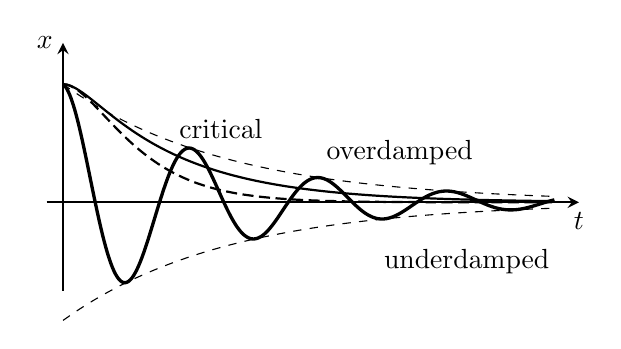
\begin{tikzpicture}[x=0.52cm,y=1.5cm,>=stealth]
  \draw[thick,->] (-0.4,0) -- (12.6,0) node[below] {$t$};
  \draw[thick,->] (0,-0.75) -- (0,1.35) node[left] {$x$};
  \draw[dashed,domain=0:12,samples=120,variable=\t] plot ({\t},{exp(-0.25*\t)});
  \draw[dashed,domain=0:12,samples=120,variable=\t] plot ({\t},{-exp(-0.25*\t)});
  \draw[very thick,domain=0:12,samples=300,variable=\t]
       plot ({\t},{exp(-0.25*\t)*cos(2*\t r)});
  \draw[thick,dash pattern=on 4pt off 2pt,domain=0:12,samples=120,variable=\t]
       plot ({\t},{(1+\t)*exp(-\t)});
  \draw[thick,domain=0:12,samples=120,variable=\t]
       plot ({\t},{1.2*exp(-0.4*\t)-0.2*exp(-2.4*\t)});
  \node[right] at (6.2,0.42) {overdamped};
  \node[right] at (2.6,0.62) {critical};
  \node[right] at (7.6,-0.5) {underdamped};
\end{tikzpicture}
\end{center}

$b^{2} < 4mk$ হলে মূল দুটি জটিল, তাই দোলন হয় কিন্তু বিস্তার $e^{-bt/2m}$
হারে কমে; ছবিতে ভাঙা রেখা দুটিই সেই খাম (envelope)। $b^{2} > 4mk$ হলে মূল দুটি বাস্তব ও
ঋণাত্মক, দোলনই হয় না, ব্যবস্থাটি ধীরে ধীরে স্থিরাবস্থায় ফিরে আসে। ঠিক মাঝখানে
$b^{2} = 4mk$ হলে পুনরাবৃত্ত মূল, আর সেটিই সবচেয়ে দ্রুত স্থিরাবস্থায় ফিরে আসার ব্যবস্থা;
দরজার ক্লোজার বা গাড়ির shock absorber এই অবস্থার কাছাকাছি রাখা হয়।

\begin{example}
১৩ নম্বর অধ্যায়ে পাওয়া গিয়েছিল যে ছোট কোণে দোলকের প্রত্যয়নী বল
$F \approx -\dfrac{mg}{L}x$। সমীকরণটি লিখে সমাধান করো এবং পর্যায়কাল নির্ণয়
করো।
\end{example}

\begin{solbox}
Newton-এর দ্বিতীয় সূত্র:
\[
  m\ddot{x} = -\frac{mg}{L}x
  \;\Longrightarrow\; \ddot{x} + \frac{g}{L}x = 0 .
\]
এটি সরল দোলগতির সমীকরণ, যেখানে $\omega_{0}^{2} = \dfrac{g}{L}$। সুতরাং
\[
  x(t) = R\cos\left( \omega_{0}t - \varphi \right), \qquad
  T = \frac{2\pi}{\omega_{0}} = 2\pi\sqrt{\frac{L}{g}} .
\]
লক্ষ করো, $T$-তে ভর নেই এবং বিস্তারও নেই। ভর না থাকার কারণ সমীকরণেই দেখা
যাচ্ছে: $m$ দুই পাশে কাটাকাটি গেছে। বিস্তার না থাকার কারণ রৈখিকতা; আর সেই
রৈখিকতা এসেছে $\sin\theta \approx \theta$ আসন্নীকরণ থেকে (১৩ নম্বর
অধ্যায়)। বড় কোণে সমীকরণটি $\ddot{\theta} + \dfrac{g}{L}\sin\theta = 0$,
যা অরৈখিক, এবং তখন পর্যায়কাল বিস্তারের উপর নির্ভর করে।
\end{solbox}

\prob{3} একটি $RC$ বর্তনীতে ধারকের আধান $Q$ নিচের নিয়ম মেনে চলে
\[
  R\frac{dQ}{dt} + \frac{Q}{C} = 0, \qquad Q(0) = Q_{0} .
\]
সমাধান করো, এবং আধান অর্ধেক হতে কত সময় লাগে তা নির্ণয় করো।

\begin{sol}
সাজিয়ে $\dfrac{dQ}{dt} = -\dfrac{Q}{RC}$, যা ক্ষয়ের সমীকরণ। চলক পৃথক করে
\[
  \frac{dQ}{Q} = -\frac{dt}{RC}
  \;\Longrightarrow\; \ln|Q| = -\frac{t}{RC} + C_{1}
  \;\Longrightarrow\; Q = Q_{0}e^{-t/RC} .
\]
অর্ধেক হওয়ার সময়: $e^{-t/RC} = \tfrac{1}{2}$ দেয়
\[
  t = RC\ln 2 .
\]
১০ নম্বর অধ্যায়ের অর্ধায়ুর সূত্র $T_{1/2} = \dfrac{\ln 2}{\lambda}$-এর
সঙ্গে মিলিয়ে দেখো: এখানে $\lambda = \dfrac{1}{RC}$, তাই উত্তর একই। রাশি
আলাদা, সমীকরণ এক, তাই উত্তরও এক।
\end{sol}

\prob{4} $\ddot{x} + \omega_{0}^{2}x = 0$ সমীকরণটি $x(0) = x_{0}$,
$\dot{x}(0) = 0$ শর্তে সমাধান করো। এরপর দুই পাশকে $\dot{x}$ দিয়ে গুণ করে
এবং একবার integrate করে শক্তির নিত্যতা বের করো।

\begin{sol}
সাধারণ সমাধান $x = A\cos\omega_{0}t + B\sin\omega_{0}t$। শর্ত থেকে
$x(0) = A = x_{0}$ এবং $\dot{x}(0) = B\omega_{0} = 0$, অর্থাৎ $B = 0$।
সুতরাং
\[
  x(t) = x_{0}\cos\omega_{0}t .
\]

শক্তি: দুই পাশকে $\dot{x}$ দিয়ে গুণ করি:
\[
  \dot{x}\ddot{x} + \omega_{0}^{2}x\dot{x} = 0 .
\]
এবার লক্ষ করো যে chain rule অনুযায়ী
$\dfrac{d}{dt}\left( \tfrac{1}{2}\dot{x}^{2} \right) = \dot{x}\ddot{x}$ এবং
$\dfrac{d}{dt}\left( \tfrac{1}{2}x^{2} \right) = x\dot{x}$। তাই সমীকরণটি
দাঁড়ায়
\[
  \frac{d}{dt}\left[ \frac{1}{2}\dot{x}^{2}
  + \frac{1}{2}\omega_{0}^{2}x^{2} \right] = 0 ,
\]
অর্থাৎ বন্ধনীর ভেতরের রাশিটি ধ্রুবক। $m$ দিয়ে গুণ করলে সেটি
$\tfrac{1}{2}m\dot{x}^{2} + \tfrac{1}{2}kx^{2}$, অর্থাৎ গতিশক্তি ও
স্থিতিশক্তির যোগফল।

এই কৌশলটি মনে রাখার মতো: $\ddot{x} = f(x)$ ধরনের যেকোনো সমীকরণে $\dot{x}$
দিয়ে গুণ করে integrate করলে একটি সংরক্ষিত রাশি বেরিয়ে আসে। শক্তির নিত্যতা
আসলে একটি গাণিতিক কৌশলেরই ভৌত নাম।
\end{sol}

\prob{5} ক্ষয়িষ্ণু দোলন $m\ddot{x} + b\dot{x} + kx = 0$।
\begin{enumerate}
  \item Characteristic equation লিখে তিনটি ক্ষেত্র $b^{2}$ ও $4mk$-এর তুলনায়
        আলাদা করো।
  \item স্বল্প-ক্ষয়ের ক্ষেত্রে ($b^{2} < 4mk$) সাধারণ সমাধান লেখো এবং
        দোলনের কৌণিক কম্পাঙ্ক ও বিস্তারের ক্ষয়হার নির্ণয় করো।
  \item ক্ষয়িষ্ণু কম্পাঙ্ক $\omega_{0}$-এর চেয়ে বড় না ছোট, এবং কেন?
\end{enumerate}

\begin{sol}
\begin{enumerate}
  \item $m\lambda^{2}+b\lambda+k = 0$, তাই
        $\lambda = \dfrac{-b \pm \sqrt{b^{2}-4mk}}{2m}$।

        $b^{2} > 4mk$: দুটি আলাদা বাস্তব ঋণাত্মক মূল, দোলন নেই
        (overdamped)।

        $b^{2} = 4mk$: পুনরাবৃত্ত মূল $\lambda = -\dfrac{b}{2m}$, সমাধান
        $(A+Bt)e^{-bt/2m}$ (critically damped)।

        $b^{2} < 4mk$: জটিল মূল, দোলন সহ ক্ষয় (underdamped)।
  \item জটিল ক্ষেত্রে
        \[
          \lambda = -\frac{b}{2m} \pm i\omega_{d}, \qquad
          \omega_{d} = \frac{\sqrt{4mk-b^{2}}}{2m}
          = \sqrt{\frac{k}{m} - \frac{b^{2}}{4m^{2}}} .
        \]
        সুতরাং
        \[
          x(t) = e^{-bt/2m}\left( A\cos\omega_{d}t + B\sin\omega_{d}t \right) .
        \]
        দোলনের কৌণিক কম্পাঙ্ক $\omega_{d}$, আর বিস্তার $e^{-bt/2m}$ হারে
        কমে, অর্থাৎ ক্ষয় ধ্রুবক $\dfrac{2m}{b}$।
  \item $\omega_{d} = \sqrt{\omega_{0}^{2} - \dfrac{b^{2}}{4m^{2}}}
        < \omega_{0}$, অর্থাৎ ছোট। বাধা থাকলে দোলন কেবল ক্ষয়ই পায় না, একটু
        ধীরও হয়ে যায়। $b \to 0$ নিলে $\omega_{d} \to \omega_{0}$, যা
        প্রত্যাশিত।
\end{enumerate}
\end{sol}

\prob{5} চালিত দোলন: $\ddot{x} + \omega_{0}^{2}x =
\dfrac{F_{0}}{m}\cos\omega t$।
\begin{enumerate}
  \item ১৮ নম্বর অধ্যায়ের জটিল পদ্ধতি ব্যবহার করে একটি বিশেষ সমাধান
        নির্ণয় করো।
  \item বিস্তার $\omega$-এর উপর কীভাবে নির্ভর করে, এবং $\omega \to
        \omega_{0}$ হলে কী ঘটে?
\end{enumerate}

\begin{sol}
\begin{enumerate}
  \item জটিল সমীকরণটি বিবেচনা করি:
        \[
          \ddot{z} + \omega_{0}^{2}z = \frac{F_{0}}{m}e^{i\omega t} ,
        \]
        যেখানে $x = \operatorname{Re}z$। এটি বৈধ কারণ সমীকরণটি বাস্তব সহগের
        ও রৈখিক, তাই বাস্তব অংশ নিলে মূল সমীকরণ ফিরে আসে।

        চেষ্টা করি $z = Ce^{i\omega t}$। তখন
        $\ddot{z} = -\omega^{2}Ce^{i\omega t}$, তাই
        \[
          C\left( \omega_{0}^{2} - \omega^{2} \right)e^{i\omega t}
          = \frac{F_{0}}{m}e^{i\omega t}
          \;\Longrightarrow\;
          C = \frac{F_{0}}{m\left( \omega_{0}^{2}-\omega^{2} \right)} .
        \]
        $C$ বাস্তব, তাই বাস্তব অংশ নিয়ে
        \[
          x_{p}(t) = \frac{F_{0}}{m\left( \omega_{0}^{2}-\omega^{2} \right)}
          \cos\omega t .
        \]
        ১৮ নম্বর অধ্যায়ে বলা হয়েছিল যে $e^{i\omega t}$-এর derivative
        নেওয়া মানে কেবল $i\omega$ দিয়ে গুণ করা; সেই কারণেই differential
        equation-টি এখানে নিছক একটি বীজগণিতের সমীকরণে নেমে এল।
  \item বিস্তার $\left| C \right| = \dfrac{F_{0}}
        {m\left| \omega_{0}^{2}-\omega^{2} \right|}$। $\omega \to \omega_{0}$
        হলে হর শূন্যের দিকে যায় এবং বিস্তার অসীমের দিকে; এটিই অনুনাদ
        (resonance)।

        বাস্তবে বিস্তার অসীম হয় না, কারণ সব ব্যবস্থাতেই কিছু বাধা থাকে।
        $b\dot{x}$ পদটি রাখলে হরে একটি অতিরিক্ত পদ যোগ হয় এবং শিখরটি সসীম
        উচ্চতায় থেমে যায়; বাধা যত কম, শিখর তত উঁচু ও সরু।
\end{enumerate}
\end{sol}

\begin{center}
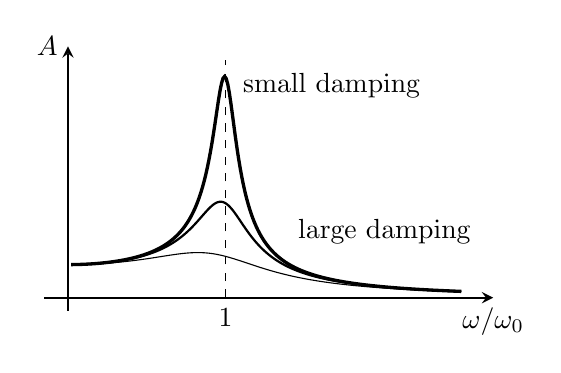
\begin{tikzpicture}[x=2.0cm,y=0.42cm,>=stealth]
  \draw[thick,->] (-0.15,0) -- (2.7,0) node[below] {$\omega/\omega_{0}$};
  \draw[thick,->] (0,-0.4) -- (0,7.6) node[left] {$A$};
  \draw[very thick,domain=0.02:2.5,samples=250,variable=\u]
    plot ({\u},{1/sqrt((1-\u*\u)*(1-\u*\u)+0.15*0.15*\u*\u)});
  \draw[thick,domain=0.02:2.5,samples=250,variable=\u]
    plot ({\u},{1/sqrt((1-\u*\u)*(1-\u*\u)+0.35*0.35*\u*\u)});
  \draw[thin,domain=0.02:2.5,samples=250,variable=\u]
    plot ({\u},{1/sqrt((1-\u*\u)*(1-\u*\u)+0.8*0.8*\u*\u)});
  \draw[dashed] (1,0) -- (1,7.2);
  \node[below] at (1,-0.05) {$1$};
  \node[right] at (1.05,6.4) {small damping};
  \node[right] at (1.4,2.0) {large damping};
\end{tikzpicture}
\end{center}

ছবিটি বাধাসহ চালিত দোলনের বিস্তার বনাম চালক কম্পাঙ্ক। তিনটি বক্ররেখা তিনটি
বাধার মানের জন্য; বাধা কমলে শিখর উঁচু ও সরু হয়, আর বাধা শূন্যের দিকে গেলে
শিখরটি উপরের সমস্যার অসীমে পরিণত হয়। সেতু, বাদ্যযন্ত্র, রেডিও টিউনিং, সবই
এই একটি ছবির উপর দাঁড়িয়ে।

\end{document}